\documentclass[a4paper, 12pt]{article}
\usepackage{general}
\usepackage{dsfont}
\title{\vspace{-8ex}A short note about differential geometry\vspace{-1ex}}
\author{Michael L{\o}iten}
\date{\vspace{-2ex}\today}

\pagestyle{fancy}
\fancyhf{}
\lhead{Differential geometry}
\chead{}
\rhead{\today}
\cfoot{\thepage}
\renewcommand{\sectionmark}[1]{\markright{#1}{}}

%===================================================
\everymath{\displaystyle}
\usepackage{titlesec}
%\titleformat*{\section}{\bfseries}%\vspace{-0.2cm}}


% Section without numbering
%\renewcommand\thesection{\hspace{-0.5cm}}
%===================================================

\renewcommand{\arraystretch}{0.8}

% References
\def\divurl{http://physicspages.com/index-physics-relativity/dinverno-introducing-einsteins-relativity-problems/}
\def\cotan{https://www.physicsforums.com/threads/basis-for-tangent-space-and-cotangent-space.283108/}
\def\NASAintro{http://www.grc.nasa.gov/WWW/k-12/Numbers/Math/documents/Tensors_TM2002211716.pdf}

\begin{document}
\maketitle

This note aims to introduce the basics of differential geometry, so that it can
easily be used in the daily work of engineers and phycisists. As differential
geometry can be a bit hard to grasp at first, the reader is also referred to
NASA's introductory text:
\href{\NASAintro
}{An Introduction to Tensors for Students of Physics and Engineering}, but note 
that $\ve{v}=(\ve{v}\cdot\ve{e}_i)\ve{e}^i = v_i\ve{e}^i$ in this note, whereas 
the authors of NASAs notes uses the notation $\ve{v}=v^i\ve{e}^i$.


\section{Manifold}
A \emph{manifold} is a topological space%
\footnote{A topological space may be defined as a set of points, along with a
          set of neighborhoods for each point, that satisfy a set of axioms
          relating points and neighborhoods.}%
, where each point satisfying the condition that the space of the manifold near
that point resembles Euclidean (flat space). The number $n$ of dimensions needed
to define a manifold is the number of parameters needed to locate all the points
on it.\\
\\
Example:\\
A geometric object such as a sphere in $\mathbb{R}^3$ is a 2D manifold. The
geometric object is nothing but a collection of points. The sphere is thus the
locus of points with equal distance to the center. This sphere is a 2D
manifold, as it needs two parameters to trace out the surface (all the points of
the manifold). We can describe a sphere by using the spherical
\emph{coordinates} (see section \ref{sec:coord}) $r$, $\theta$ and $\phi$. These
coordinates can be written in terms of the Cartesian coordinates $x$, $y$ and
$z$ as described by equation (\ref{eq:r} - \ref{eq:phi})

\begin{minipage}{0.49\textwidth}
 \begin{align}
 &r = \sqrt{x^2+y^2+z^2} \label{eq:r}\\
 &\theta = \cos\L(\frac{z}{\sqrt{x^2+y^2+z^2}}\R) \label{eq:theta}\\
 &\phi = \tan\L(\frac{y}{x}\R) \label{eq:phi}
 \end{align}
\end{minipage}
\begin{minipage}{0.49\textwidth}
 \begin{align}
 &x = r\sin(\theta)\cos(\phi) \label{eq:x}\\
 &y = r\sin(\theta)\sin(\phi) \label{eq:y}\\
 &z = r\cos(\theta) \label{eq:z}
 \end{align}
\end{minipage}
%
The Cartesian coordinates written in terms of the spherical coordinates (the
inverse transformation) is found from equation (\ref{eq:x} - \ref{eq:z}),
where $\theta \in [0,\pi)$ and $\phi \in [0,2\pi)$.

The sphere (or rather the locus of all points making the sphere) is found
by fixing $r$, and let $\theta$ and $\phi$ run over all points (see figure
\ref{fig:sphere}). Note that these points can be written in both the Cartesian
and the spherical coordinate system. In general, a \emph{coordinate
(hyper)surface} is the (hyper)surface one get if one holds one of the
coordinates constant, and let all the other variables vary. %
\footnote{In the example of a sphere: $\theta$ and $\phi$ can take all
	  possible values in the domain, even though not all combinations of
	  $x$, $y$ and $z$ are allowed due to the constraint.}%
%
A \emph{coordinate curve} is the collection of point one gets by intersection of
two coordinate (hyper)surfaces.

Note that the sphere itself is non-Euclidean, but small enough parts of it is.
An often used analogy is to say that although the earth is not flat, it may
sometimes appear somewhat flat to us since we are so small compared to the
earth.

In \emph{constraint} form the sphere can be written as
%
\begin{align*}
 x^2+y^2+z^2-r^2 = 0
\end{align*}
%
If we have $m$ dimensions in the subsurface embedded in an $n$-dimensional
manifold, we must have $n-m$ constraints.
%
\begin{figure}[h!]
\center
 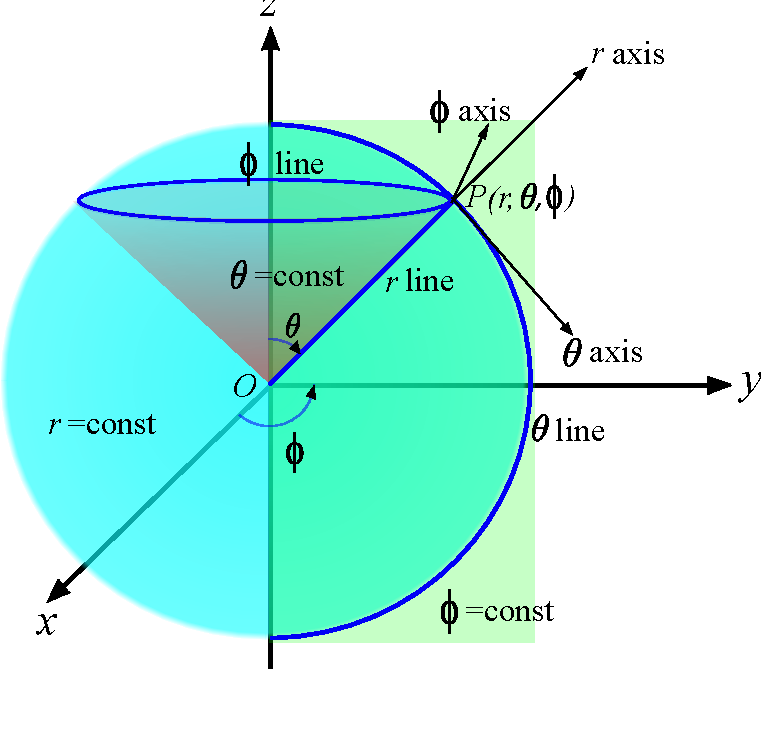
\includegraphics[width=0.5\textwidth]{figures/Spherical_coordinate_elements}
 \caption{Coordinate curves and coordinate surfaces of the spherical
	  coordinate system.}
 \label{fig:sphere}
\end{figure}





\section{Coordinates} \label{sec:coord}
$x$, $y$ and $z$ in equation (\ref{eq:x} - \ref{eq:z}) are called
\emph{coordinates}. A coordinate system is a set of $n$ variables which fix a
geometric object.

Each point on a $n$-dimensional manifold possesses a set of
$n$ coordinates. Coordinate systems which covers only a part of the manifold is
called a \emph{coordinate patch}. A set of coordinate patches that covers the
whole manifold is called an \emph{atlas}. The theory of manifolds tells us how
to get from one coordinate patch to another by a coordinate transformation in
the overlap region.

We can describe curvilinear coordinates in a mathematical language: A
curvilinear coordinate system is simply a coordinate patch on the differentiable
manifold $\mathbb{E}^n$ ($n$-dimensional Euclidean space) that is diffeomorphic
%
\footnote{Diffeomorphism is an isomorphism\footnotemark of smooth manifolds.}%
\footnotetext{An isomorphism is a homomorphism\footnotemark(or more generally a
              morphism\footnotemark) that admits an inverse.}%
\footnotetext[3]{A homomorphism is a structure-preserving map between two
                 algebraic structures (such as groups, rings, or vector
                 spaces).}%
\footnotetext{Morphism refers to a structure-preserving map from one
              mathematical structure to another(generalizes the idea of
	      a function).}%
%
to the Cartesian coordinate patch on the manifold.







\section{Change of coordinates} \label{sec:change_of_coordinates}
In general the change of coordinates $x^a \to x'^a$ is given by
%
\begin{align}
 (x')^a = f^a(x^1,x^2,\ldots,x^n)\qquad a\in{1,2,\ldots,n} \label{eq:transform}
\end{align}
%
where the $f$'s are single valued, continuous differentiable function for
certain ranges of their arguments. Notice that the superscript in equation
(\ref{eq:transform}) does not refer to taking powers, but rather to components
of a contravariant tensor, and that the dangerous notation $(x')^a =
x^a(x^1,x^2,\ldots,x^n)$ often is used.


\begin{example}{Change of basis}
 If we know how the bases relative to each other, for example
 %
 \begin{align}
  &\ve{a}_1=\frac{1}{\sqrt{2}}(\ve{b}_1 + \ve{b}_2)&
  &\ve{a}_2=3\ve{b}_2
  \label{eq:eq_with_basis_vector}
 \end{align}
 %
 We can write
 %
 \begin{align*}
  [\ve{v}]_b &= A_{a\to b}[\ve{v}]_a\\
  %
  %
  \begin{bmatrix}
   v_{1,b}\\
   v_{2,b}
  \end{bmatrix}_b
  &=
   \begin{bmatrix}
   [\ve{a}_1]_b & [\ve{a}_2]_b
  \end{bmatrix}_{a\to b}
    \begin{bmatrix}
   v_{1,a}\\
   v_{2,a}
  \end{bmatrix}_a\\
  %
  %
  \begin{bmatrix}
   v_{1,b}\\
   v_{2,b}
  \end{bmatrix}_b
  &=
   \begin{bmatrix}
   \frac{1}{\sqrt{2}} & 0\\
   \frac{1}{\sqrt{2}} & 3
  \end{bmatrix}_{a\to b}
    \begin{bmatrix}
   v_{1,a}\\
   v_{2,a}
  \end{bmatrix}_a\\
  %
  %
  v_{1,b} &= \frac{1}{\sqrt{2}}v_{1,a}
  \numberthis \label{eq:coord_v1b}\\
  v_{2,b} &= \frac{1}{\sqrt{2}}v_{1,a} + 3v_{2,a}
  \numberthis \label{eq:coord_v2b}
 \end{align*}
\end{example}
%
The example here was in rectilinear coordinates (so there is no difference
between co- and contravariant tensors), but in general (and for contravariant
vectors), we have that%
\footnote{We will here use index notation (which means that the individual
          tensors in an expression gets individual indices) with the Einstein
          summation rule (when an index variable appears once as upper index
          and once as lower index in a single term (called a dummy index) it
          implies summation of that term over all the values of the index).}
%
\begin{align}
 A_{\text{unprimed}\to \text{primed}}
 =
 \begin{bmatrix}
  \parti{(x')^i}{x^j}
 \end{bmatrix}
 \label{eq:contravariant_matrix}
\end{align}
%
Where equation (\ref{eq:contravariant_matrix}) is a matrix with the $x$'s
referring to the different coordinates. The \emph{Jacobian} is
defined as $J\defined|A_{\text{unprimed}\to \text{primed}}|$. A requirement for
having a inverse transformation is that $J$ is non-zero in the point under
consideration. We further have that the matrix inverse of the Jacobian matrix
of an invertible function is the Jacobian matrix of the inverse function, which
means that
%
$\begin{bmatrix}
 \parti{(x')^i}{x^j}
\end{bmatrix}^{-1}$
has the determinant $1/J$. Note that
%
\begin{align*}
 \parti{x^i}{(x')^j} \neq \L[\parti{(x')^j}{x^i}\R]^{-1}
\end{align*}
%
as explained in section \ref{sec:metrics}.

\vspace{0.5cm}
\begin{greenbox}{Mnemonic: $(A_{x \to x'})_{i,j} = \parti{x^i}{(x')^j}$ (only
contravariant)}
 A way to remember what are the rows and columns if we want to write $A_{x \to
 x'}$ as a matrix, is to remember that the $i$ denotes the rows number and
 $j$ denotes column number in $A_{i,j}$.

 Note that applies only for the contravariant transfomation (see section
\ref{sec:co-cont}, or example \hyperref[ex:fmt]{4} ). In general one must look
at the summed index in order to decide how to write the matrix in a matrix
product.
\end{greenbox}

\begin{example}{Vector field transformation by using the transformation matrix}
 \label{ex:vft}
 Let's assume we have a (contravariant) vector given in the basis
$\{\hv{e}_\rho,
 \hv{e}_\phi, \hv{e}_z\}$, and would like to express it in the Cartesian basis
 $\{\hv{e}_x, \hv{e}_y, \hv{e}_z\}$. The transformation equations (the
coordinates
 written as a function of the other coordinates) read
 %
 \begin{align*}
  &x = \rho \cos\phi&
  &\rho = \sqrt{x^2+y^2}&
  \\
  &y = \rho \sin\phi&
  &\phi = \atan\L(\frac{y}{x}\R)&
  \\
  &z=z&
  &z=z&
 \end{align*}
 %
 Note that
 %
 \begin{align}
  \ve{A} =
  A_x \hv{e}_x + A_y \hv{e}_y + A_z \hv{e}_z =
  A_\rho \hv{e}_\rho + A_\phi \hv{e}_\phi + A_z  \hv{e}_z
  \label{eq:component}
 \end{align}
 %
 So if we know how the $\hv{e}_x$, $\hv{e}_y$ and $\hv{e}_z$ can be written in
terms
 of $\hv{e}_\rho$, $\hv{e}_\phi$ and $\hv{e}_z$, we can simply write the
components
 in the new coordinate system to complete the transformation. We will here use
 the notation $_{\{\hv{x}_1, \hv{x}_2, \hv{x}_3\}} \ve{A}$, meaning the vector
 $\ve{A}$ described in the basis ${\{\hv{x}_1, \hv{x}_2, \hv{x}_3\}}$.

 Let us try to use (\ref{eq:contravariant_matrix}). We get
 %
 \begin{align*}
  _{\{\hv{e}_x, \hv{e}_y, \hv{e}_z\}} \ve{A}
   =
   \L[\parti{(x, y, z)}{(\rho, \phi, z)}\R] \;
    _{\{\ve{e}_\rho, \ve{e}_\phi,\ve{e}_z\}}\ve{A}
   = \begin{bmatrix} \cos\phi & -\rho\sin\phi & 0 \\
                     \sin\phi &  \rho\cos\phi & 0 \\
                     0 & 0 & 1
  \end{bmatrix} \;
  _{\{\ve{e}_\rho, \ve{e}_\phi,\ve{e}_z\}}\ve{A}
 \end{align*}
 %
 If we try to transform $\ve{e}_\phi$, we get
 %
 \begin{align*}
   \begin{bmatrix} \cos\phi & -\rho\sin\phi & 0 \\
                     \sin\phi &  \rho\cos\phi & 0 \\
                     0 & 0 & 1
  \end{bmatrix}
  \begin{bmatrix} 0 \\
 		 1 \\
 		 0 \\
  \end{bmatrix}
  =
  \begin{bmatrix} -\rho\sin\phi \\
 		 \rho\cos\phi \\
 		 0 \\
  \end{bmatrix}
 \end{align*}
 %
 Meaning that
 %
 \begin{align*}
  \ve{e}_\phi = -\rho\sin\phi \hv{e}_x + \rho\cos\phi \hv{e}_y
 \end{align*}
 %
 We see that this vector has length $\rho$, but we wanted to transform from
 something written in a unit basis (where all the basis vectors has length
$1$).
 To ensure this we must normalize the columns in the transformation matrix to
 one, in other words, we must use
 %
 \begin{align*}
   \L[
      \frac{\displaystyle \parti{(x, y, z)}{\phi}}{
            \displaystyle \L\|\parti{(x,y, z)}{\phi}\R\| } \R]
 \end{align*}
 %
 for each column in the transformation matrix. We will use the notation
 %
 \begin{align*}
   \L[
      \frac{\displaystyle \parti{(x, y, z)}{(\rho, \phi, z)}}{
            \displaystyle \L\|\parti{(x,y, z)}{(\rho, \phi, z)}\R\| } \R]
 \end{align*}
 %
 to denote that all the columns in the transformation matrix is normalized.
With
 this notation, we finally get that
 %
 \begin{align*}
  _{\{\hv{e}_x, \hv{e}_y, \hv{e}_z\}} \ve{A}
   =
     \L[
      \frac{\displaystyle \parti{(x, y, z)}{(\rho, \phi, z)}}{
            \displaystyle \L\|\parti{(x,y, z)}{(\rho, \phi, z)}\R\| } \R] \;
    _{\{\hv{e}_\rho, \hv{e}_\phi,\hv{e}_z\}}\ve{A}
   = \begin{bmatrix} \cos\phi & -\sin\phi & 0 \\
                     \sin\phi &  \cos\phi & 0 \\
                     0 & 0 & 1
  \end{bmatrix} \;
  _{\{\hv{e}_\rho, \hv{e}_\phi,\hv{e}_z\}}\ve{A}
 \end{align*}
\end{example}





\section{Co- and contravariant vectors}\label{sec:co-cont}
A basis is spanning the space and needs (in general) to be evaluated at each
point in the space. It can be thought of as a set of reference axes.
A change of scale on the reference axes corresponds to a change of units in the
problem. For instance, in changing scale from meters to centimeters (that is,
dividing the scale of the reference axes by $100$), the components of a
measured velocity vector will multiply by $100$.

For a vector (such as a direction vector or velocity vector) to be
basis-independent, the components of the vector must contra-vary with a change
of basis to compensate. The components of vectors (as opposed to those of dual
vectors) are said to be contravariant. Examples of vectors with contravariant
components include the position of an object relative to an observer, or any
derivative of position with respect to time.

For a dual vector (also called a convector) to be basis-independent, the
components of the dual vector must co-vary with a change of basis to remain
representing the same convector. Examples of covariant vectors generally appear
when taking a gradient of a function.





\subsection{Contravariant tensors}
A contravariant vector (that is a tensor of rank $1$) is defined by a vector
which transforms as
%
\begin{align*}
 (A')^i = \parti{(x')^i}{x^j} A^j
\end{align*}
%
A higher rank tensor will transform as
%
\begin{align*}
 (A')^{ab\ldots} = \parti{(x')^{a}}{x^{c}}\parti{(x')^{b}}{x^{d}}\ldots
A^{cd\ldots}
\end{align*}
%

\vspace{0.5cm}
\begin{greenbox}{Mnemonic: Contravariant components $= \; \uparrow$}
 The indices in the components are up, and the primed quantity is on
top in the partial differential, since the ``n'' in ``contravariant'' can be
thought of as a arrow pointing up. The primed quantities are written with the
same index.
\end{greenbox}
%
\subsubsection{Why the coordinates in equation (\ref{eq:transform}) are with
superscript}
Consider two neighboring points $P$ and $Q$ on a manifold with coordinates
$x^a$ and $x^a + \text{d}x^a$. The infinitesimal vector $\ve{PQ} =
\text{d}x^a$, is attached to $P$. The components in another coordinate system
$x'^a=x'^a(x^a)$ can be found by using the chain rule
%
\begin{align}
 \text{d}(x')^a = \parti{(x')^a}{x^b}\text{d}x^b \label{eq:infinitesimal_vec}
\end{align}
%
and hence are components of equation (\ref{eq:transform}) written
contravariantly. Note that the vectors in equation (\ref{eq:infinitesimal_vec})
are nothing but a specials cases of general vectors, and that one can always
find the transformation by using the chain rule.



\subsection{Covariant tensors}
Covariant vectors are defined by transforming as
%
\begin{align*}
 (A')_i = \parti{x^j}{(x')^i} A_j
\end{align*}
%
A higher rank tensor will transform as
%
\begin{align*}
 (A')_{ab\ldots} = \parti{x^{c}}{(x')^{a}}\parti{x^{d}}{(x')^{b}}\ldots
A_{cd\ldots}
\end{align*}
%
Note that differentiation of $\phi=\phi(x^b(x'))$ with respect to $(x')^a$
gives the contravariant transformation matrix as
$\parti{\phi}{(x')^a}=\parti{x^b}{(x')^a}\parti{\phi}{x^b}$ due to the chain
rule. Note that it is always possible to use the chain rule in order to get
the transformation\label{foot:phi}.

\vspace{0.5cm}
\begin{greenbox}{Mnemonic: Covariant components $= \; \downarrow$}
 The indices in the components are down, and the primed quantity is
 in the lower part of the partial differential, since the ``v'' in
 ``covariant'' can be thought of as an arrow pointing downwards. Note
 that the coordinates in the transformation matrix still have an upper
 index. The primed quantities are written with the same index.
\end{greenbox}


\subsection{Mixed tensors}
A mixed tensor transforms as
%
\begin{align*}
 (A')^{ab\ldots}_{\qquad cd\ldots} =
 \parti{(x')^{a}}{x^{e}}\parti{(x')^{b}}{x^{f}}\ldots
 \parti{x^{g}}{(x')^{c}}\parti{x^{h}}{(x')^{d}}\ldots
  A^{ef\ldots}_{\qquad gh\ldots}
\end{align*}
%
Note the notation, and that $A^{ab\ldots}_{\qquad cd\ldots} \neq
A^{\qquad ab\ldots}_{cd\ldots}$ as $\ve{e}^a\ve{e}_c \neq \ve{e}_a\ve{e}^c$ in
general, and that tensors such as $A^{a\ldots \quad c\ldots}_{\quad b\ldots}$
exist.

At last, it is worth mentioning that any tensor equation (such as
$X_{ab}=Y_{ab}$) holds true in \textbf{every} coordinate system.




\section{Pseudotensors}
Up until this point we have only considered polar vectors, which transformed to
its negative under inversion of its coordinate axes. There is another type of
vectors called \emph{pseudovectors} or \emph{axial} vectors which are invariant
under inversion. Whereas polar tensors transforms as
%
\begin{align*}
 \ve{A}' = \ve{S}\ve{A}
\end{align*}
%
pseudotensors transforms as
%
\begin{align*}
 \ve{A}' = \det(\ve{A})\ve{S}\ve{A}
\end{align*}
%
Examples of pseudovectors include angular velocity vector $\ve{\omega}$,
angular momentum $\ve{L}$ and torque $\ve{\tau}$. All of these are defined
from a cross product. We have that
%
\begin{align*}
 \text{vector} \times \text{vector} &= \text{pseudovector}\\
 \text{pseudovector} \times \text{pseudovector} &= \text{pseudovector}\\
 \text{pseudovector} \times \text{vector} &= \text{vector}\\
 \text{vector} \times \text{pseudovector} &= \text{vector}\\
\end{align*}
%
However $\ve{B}$ is also a pseudovector. One can convince oneself of that by
knowing that $\ve{v}$ and $F$ is a polar vector when looking at the Lorentz
force%
\footnote{Note: The sum of a polar vector with a pseudovector is neither a
polar vector nor a pseudovector, and behaves rather strange under rotation.
Such vectors can occur, for example when calculating decay due to the weak
interaction.}%
.




\section{Basis vectors and metrics}
In general a vector can be written as
%
\begin{align*}
 \ve{A} = A^i\ve{e}_i = A_i\ve{e}^i
\end{align*}
%
And a second rank tensor can be written in four different ways
%
\begin{align*}
 \ve{A} =
 A^{ij}\ve{e}_i\ve{e}_j =
 A_{ij}\ve{e}^i\ve{e}^j =
 A^{i}_{\;\;j}\ve{e}^i\ve{e}_j =
 A_{i}^{\;\;j}\ve{e}_i\ve{e}^j
\end{align*}
%
Where the covariant basis (transforms covariantly) can be written in operator
form (see section \ref{sec:bvdf}) as
%
\begin{align}
 \ve{e}_i = \parti{}{x^i} \label{eq:cov_basis}
\end{align}
%
and the contravariant basis (transforms contravariantly) can be written in
operator form (see section \ref{sec:bvdf}) as
%
\begin{align}
 \ve{e}^i = \text{d}x^i \label{eq:con_basis}
\end{align}
%
(see figure \ref{fig:basis}).

\vspace{0.5cm}
\begin{greenbox}{Mnemonic: $\parti{}{x^i} = $ covariant,  $\text{d}x^i = $
contravariant }
 One can remember that $\parti{}{x^i}$ is the \emph{covariant} basis vector
and that $\text{d}x^i$ is the \emph{contravariant} basis vector by realizing
that the index in $\text{d}x^i$ is located above the index in $\parti{}{x^i}$,
and therefore we can use that the ``n'' in ``contravariant'' is ``pointing up''
as described above.
\end{greenbox}


\subsection{Finding the basis vectors of a new coordinate system}
This can be done as shown in example \hyperref[ex:vft]{2}. Each column in the
Jacobian matrix is a basis vector for the new coordinate system written with
respect to the old coordinate system. Notice that this basis vector does not
necessarily have unit length.




\subsection{The derivative of a basis vector}
\subsubsection{By ``hard rewriting''}
Since the manifold can locally be written in Cartesian coordinates
(by definition), it is usually a good idea to write the basis vector back to
Cartesian coordinates, take the derivative, and transform back to the new
coordinate system. Let us elucidate this with an example:

\begin{example}{The derivative of a basis vector}
 Using the coordinate transform given in example \hyperref[ex:vft]{2}, we would
 like to calculate $\partial_\phi \ve{e}_\rho$. We have that
 %
 \begin{align*}
  \partial_\phi \ve{e}_\rho &= \partial_\phi
\L(\cos\phi\hv{e}_x+\sin\phi\hv{e}_y\R)\\
  %
    &= \L(\hv{e}_x\partial_\phi \cos\phi + \cos\phi \partial_\phi \hv{e}_x\R)
      +\L(\hv{e}_y\partial_\phi \sin\phi + \sin\phi \partial_\phi \hv{e}_y\R)\\
  %
    &= - \sin\phi\hv{e}_x + \cos\phi\hv{e}_y\\
    &= \hv{e}_\phi
 \end{align*}
 %
 Where we have used that the Cartesian
\end{example}
%


\subsubsection{By using Christoffel symbols}
Due to the fact that $\ve{e}_i$ and $\ve{e}^i$ are reciprocal vectors (see for
example the intro in the book ``Flux Coordinates and Magnetic Field Curvature''
by D'Haeseleer et al.), we have that
%
\begin{align*}
 \ve{e}_i\ve{e}^i = \ve{e}^i\ve{e}_i = \mathds{1}
\end{align*}
%
where $\mathds{1}$ is the identity tensor. Thus, we have that
%
\begin{align*}
 \parti{\ve{e}_i}{x^k} &= \L\{\parti{\ve{e}_i}{x^k} \cdot \ve{e}^j\R\} \ve{e}_j
 =  \L\{\ve{e}^j \cdot \parti{\ve{e}_i}{x^k} \R\} \ve{e}_j\\
 %
 \parti{\ve{e}^i}{x^k} &= \L[\parti{\ve{e}^i}{x^k} \cdot \ve{e}_j\R] \ve{e}^j
 =  \L[\ve{e}_j \cdot \parti{\ve{e}^i}{x^k} \R] \ve{e}^j,
\end{align*}
%
where we have used that the dot product commutes. We now introduce the
Christoffel symbol of first kind $[j, ik]$ and second kind
$
 \begin{Bmatrix}
   \,j\,\\
  i\,\,k
 \end{Bmatrix}
$
%
\begin{align*}
 \begin{Bmatrix}
   \,j\,\\
  i\,\,k
 \end{Bmatrix}
 &=  \L\{\ve{e}^j \cdot \parti{\ve{e}_i}{x^k} \R\}
 = \frac{1}{2}g^{jn}\L(\parti{g_{ni}}{x^k} + \parti{g_{nk}}{x^i} -
   \parti{g_{ik}}{x^n}\R)\\
 %
 [j,ik]
 &=\L[\ve{e}_j \cdot \parti{\ve{e}^i}{x^k} \R]
 = \frac{1}{2}\L(\parti{g_{ji}}{x^k} + \parti{g_{jk}}{x^i} -
   \parti{g_{ik}}{x^j}\R)
\end{align*}
%
where $g_{ij}=\ve{e}_i\cdot\ve{e}_j$, $g^{ij}=\ve{e}^i\cdot\ve{e}^j$ and the
last relation can be shown in a straigth forward way.






\subsection{Basis vectors in differential form}\label{sec:bvdf}
The basis vectors written in equation (\ref{eq:cov_basis}) and
(\ref{eq:con_basis}) surely doesn't look like the ``classical'' basis vectors
one encountered when first facing linear algebra. They are rather defined as
operators.

It actually makes sense if one consider the \emph{tangent space}. Let us
consider a point $P$ on our manifold (for example the sphere in the example in
section \ref{sec:coord}). If we draw all possible curves (for example
the curve $S(r,\theta,\phi)$ parametrized by $t$ [that is
$S(r,\theta,\phi) = S(r(t),\theta(t),\phi(t))$]%
%
\footnote{\label{note:curve}Note that this can be any curve going through the
          point of consideration. Do not confuse it with the coordinate curve.}%
%
) through $P$ and take the directional derivative $\Bigg($that is $\deri{S}{t}
=
\parti{S}{r}\parti{r}{t} + \parti{S}{\theta}\parti{\theta}{t} +
\parti{S}{\phi}\parti{\phi}{t}\Bigg)$ of each curve, we can generate a
collection of tangents to $P$, which is called the tangent space. Notice that
the partial derivative $\parti{S}{x^i}$ at the point is the change of the line
along the coordinate $x^i$. Thus the tuple of all $\parti{S}{x^i}$ $\Bigg($in
our case $\L\{\parti{S}{r}, \parti{S}{\theta}, \parti{S}{\phi}\R\} \Bigg)$ are
along the direction which spans the tangent space (see figure \ref{fig:basis}).
This is true for all curves $\in C^{\infty}$ (that is, smooth curves). Notice
that the partial derivative of the curve along the coordinate direction
transforms covariantly (as shown in (\ref{foot:phi})), and is independent of
the
curve $S$.

A tangent vector $\ve{X}$ (a vector living in the tangent space) can thus be
written in operator form as $\ve{X}=a^i\parti{}{x^{i}}$. The dual space to
the tangent space is called the \emph{cotangent space}. The cotangent space is
made up of all linear functionals (a function from a vector space into its
underlying scalar field [that is it takes a vector in the vector space as an
input and returns a scalar value]) on the tangent space. The i'th coordinate
function of the tangent space is defined by $\d x^i(\ve{X}) = a_i$, and thus
$\d
x^i$ makes up the dual (cotangent space) to the tangent space. It can be shown
that the cotangent basis vector in a point of a coordinate is perpendicular on
the surface spanned by holding the coordinate under consideration fixed to the
point of consideration while varying all the other coordinates. This is
depicted
in figure \ref{fig:basis}.
%
\begin{figure}[h!]
\center
 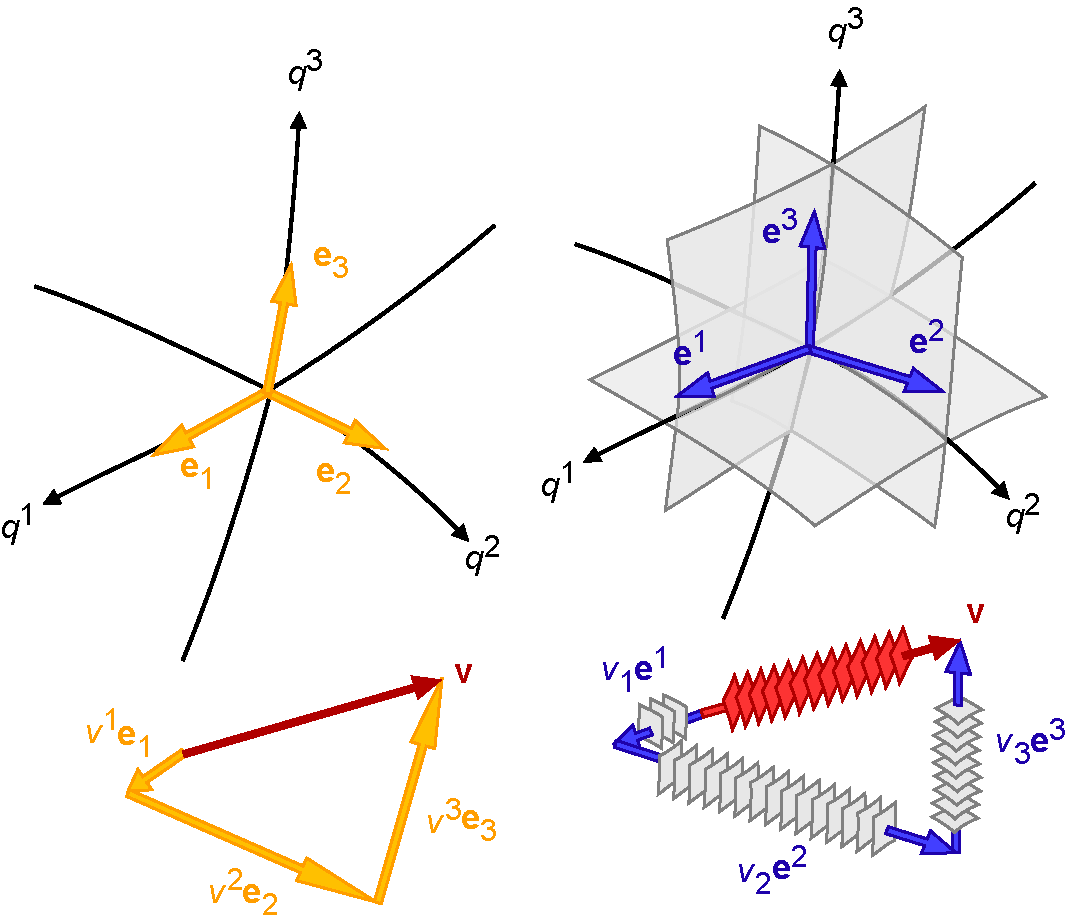
\includegraphics[width=0.5\textwidth]{figures/co-contra}
 \caption{Basis vectors in a point.}
 \label{fig:basis}
\end{figure}

\vspace{0.5cm}
\begin{greenbox}{Mnemonic: How to change unit vectors}
 Covariant unit vectors: Insert a function of a curve as a function of the new
 coordinates $(x')$ (which again can be expressed in the current coordinates
 $x$), for example the function $f((x')(x))$, and use the chain rule on the
 expression on $\parti{f((x')(x))}{x^i}$.\\
 Contravariant unit vectors: Use the chain rule of the infinitesimal.
\end{greenbox}
%
Finally, note that some authors prefer the somewhat bad notation $\ve{e}^i =
\grad u^i$ and $\ve{e}_i = \parti{\ve{R}}{u^i}$, where $\ve{R}(\ve{u})$ is a
curve\hyperref[note:curve]{$^9$}.The notation differs from what introduced
above by explicitly specifying the curve under consideration.

For the covariant basis-vectors, we observe that $\ve{e}_i = \parti{}{u^i}$
with $\ve{R}$ as the curve under consideration gives $\parti{\ve{R}}{u^i}$.

It can be a bit trickier to explain how $\grad u^i$ comes about, but if we
consider $\d u^i = \parti{u^i}{R^j} \d R^j$ as an operator, and let it operate
on the tangent $\parti{}{R^k}$, we get $\d u^i\L(\parti{}{R^k}\R) =
\parti{u^i}{R^j} \d R^j\L(\parti{}{R^k}\R) = \parti{u^i}{R^j} \delta^j_k =
\parti{u^i}{R^k}$ and define $\parti{u^i}{R^j}$ as $\nabla u^i$, we end up with
the same.





\section{The metric tensor and the Kronecker delta}\label{sec:metrics}
The Kronecker delta $\delta^i_j = 1$ if $i=j$, and zero otherwise. The
independence of the coordinates can be expressed as
%
\begin{align*}
 \delta^i_j = \parti{x^i}{x^j} = \parti{x^i[(x')^k\{x^l\}]}{x^j} =
 \parti{x^i}{(x')^k}\parti{(x')^k}{x^j},
\end{align*}
%
where $x^i$ is a function of $(x')^k$, which again is a function of $x^l$, here
written as $x^i = x^i[(x')^k\{x^l\}]$. Note that
%
\begin{align*}
 \parti{x^i}{(x')^j} \neq \L[\parti{(x')^j}{x^i}\R]^{-1}
\end{align*}


Further, from section \ref{sec:bvdf} we have that
%
\begin{align*}
 \d x^i \L(\parti{}{x^j}\R) = \ve{e}^i\cdot\ve{e}_j = \delta^i_j
\end{align*}
%
The metric tensors are defined as
%
\begin{align*}
 &g_{ij} = \ve{e}_i\cdot\ve{e}_j&
 &g^{ij} = \ve{e}^i\cdot\ve{e}^j
\end{align*}
%
and we notice that
%
\begin{align*}
 &g^{ij} g_{jk} = \delta^i_j&
 &e_i = g_{ij}e^j &
 &e^i = g^{ij}e_j&.
\end{align*}
%
\begin{example}{Finding the metric tensors}
 \label{ex:fmt}
 Let us again use cylinder coordinates.
 The contravariant metric tensor can be found from the contravariant
 basis vectors from example \hyperref[ex:vft]{2}. We find that
 %
 \begin{align*}
  g_{ij} = \ve{e}_i\cdot\ve{e}_j =
  \begin{bmatrix}
   1 & 0 & 0\\
   0 & r^2 & 0\\
   0 & 0 & 1
  \end{bmatrix}
 \end{align*}
 %
 Next, to find the covariant basis vectors, we need to find the covariant
 transformation matrix $A_{\text{unprimed}\to \text{primed}, \text{covariant}}
 = \parti{x^j}{(x')^i}$. We now need to keep our head straigth to find out how
 to represent this matrix. Shall we let $i$ denote the columns and $j$ the
 rows as we did for the contravariant matrix, or vica versa? To decide this, we
 should look at the transfomation rule. We have for covariant vectors that
 $(A')_i = \parti{x^j}{(x')^i} A_j$. Hence, there is a sum over the $j$'th
 element. If we want to form this as a matrix product, we should let let $j$
 denote the columns and $i$ denote the rows in $\parti{x^j}{(x')^i}$ if we want
 to write $\parti{x^j}{(x')^i} A_j$ as a matrix product.

 There are now two ways to find $A_{\text{unprimed}\to \text{primed},
 \text{covariant}}$. The first way is to calculate the derivates, and the
 second involves finding the inverse of the contravariant $A_{\text{unprimed}\to
 \text{primed}}$. The first way is as follows
 Finally, we have the often used relations
%
\begin{align*}
 &\det(g_{ij}) = J^2&
 &\deri{[\det(g_{ij})]}{x^k} = \det(g_{ij})g^{ij}\parti{g_{im}}{x^k}
\end{align*}
 %
 \renewcommand\arraystretch{2}
 \begin{align*}
  &A_{\text{unprimed}\to \text{primed}, \text{covariant}} =
  \parti{x^j}{(x')^i}\\
  %
  &=
  \begin{bmatrix}
   \parti{\rho}{x} & \parti{\phi}{x} & \parti{z}{x}\\
   \parti{\rho}{y} & \parti{\phi}{y} & \parti{z}{y}\\
   \parti{\rho}{z} & \parti{\phi}{z} & \parti{z}{z}
  \end{bmatrix}
  =
  \begin{bmatrix}
   \frac{x}{\sqrt{x^2+y^2}} & -\frac{y}{x^2+y^2} & 0\\
   \frac{y}{\sqrt{x^2+y^2}} & \frac{x}{x^2+y^2} & 0\\
   0 & 0 & 1
  \end{bmatrix}
  =
  \begin{bmatrix}
   \cos\phi & -\frac{\sin\phi}{\rho} & 0\\
   \sin\phi & \frac{\cos\phi}{\rho} & 0\\
   0 & 0 & 1
  \end{bmatrix}
 \end{align*}
 %
 Hence
 %
 \renewcommand\arraystretch{1}
 \begin{align*}
  \ve{e}^{\phi} =
  \begin{bmatrix}
   \cos\phi & -\frac{\sin\phi}{\rho} & 0\\
   \sin\phi & \frac{\cos\phi}{\rho} & 0\\
   0 & 0 & 1
  \end{bmatrix}
  \begin{bmatrix}
   0\\
   1\\
   0
  \end{bmatrix}
  =
  \begin{bmatrix}
   -\frac{\sin\phi}{\rho}\\
   \frac{\cos\phi}{\rho}\\
   0
  \end{bmatrix}
  =
  -\frac{\sin\phi}{\rho}\hv{e}_x + \frac{\cos\phi}{\rho}\hv{e}_y
 \end{align*}
 %
 In the second way, we find $A_{\text{unprimed}\to \text{primed},
 \text{covariant}}$ through the inverse of $A_{\text{unprimed}\to
 \text{primed}}$. It is important to note that
 %
 \begin{align*}
  A_{\text{unprimed}\to \text{primed}, \text{covariant}} =
  [(A_{\text{unprimed}\to \text{primed}})^{-1}]^T
 \end{align*}
 %
 We find then that
 %
 \begin{align*}
  g^{ij} = \ve{e}^i\cdot\ve{e}^j =
  \begin{bmatrix}
   1 & 0 & 0\\
   0 & \frac{1}{r^2} & 0\\
   0 & 0 & 1
  \end{bmatrix}
 \end{align*}
 %
 Generally, we have that $g_{ij} = (g^{ij})^{-1}$
\end{example}
%



\section{The $\nabla$ operator}
The del operator is simply defined as
%
\begin{align*}
 \nabla = \ve{e}_i \parti{}{x_i}
\end{align*}
%
from this we get that products such as $(\nabla \ve{B}) \cdot \hv{b}$ can be
written as
%
\begin{align*}
 (\nabla \ve{B}) \cdot \hv{b} =
 \ve{e}_i \parti{}{x_i} (B^j \ve{e}_j) \cdot \frac{B_k}{\|\ve{B}\|}\ve{e}^k
\end{align*}
%
Note that there exists tensor identities just like vector identities, which is
coordinate independent and makes it easy to evaluate expressions such that the
one above. We have that
%
\begin{align*}
 (\nabla \ve{B}) \cdot \hv{b} = \grad \|\ve{B}\|
\end{align*}




\section{Transformation of a vector through transformation of the basis vectors}
Let's say that we would to go from a description in Cartesian coordinates
(given by the coordinates $\ve{R}$), to a description in curvilinear (given by
the coordinates $\ve{u}$). We have that the component in the Cartesian
coordinates can be written as $(v')^i =
(v')^i(\ve{R}(\ve{u}))$, where
$\ve{R}(\ve{u}) =
 \begin{bmatrix}
  x^1(u^1,u^2,u^3)&
  x^2(u^1,u^2,u^3)&
  x^3(u^1,u^2,u^3)
 \end{bmatrix}
$
is the transformation and that the components written in the curvilinear
coordinates can be written
as
$v^i =
v^i(\ve{u}(\ve{R}))$, where
$\ve{u}(\ve{R}) =
 \begin{bmatrix}
  u^1(x^1,x^2,x^3)&
  u^2(x^1,x^2,x^3)&
  u^3(x^1,x^2,x^3)
 \end{bmatrix}
$ is the transformation. The transformation from Cartesian to curvilinear
coordinates can be written as
%
\begin{align*}
 \ve{v} &=
 (v')^i(\ve{e}')_i =
 (v')^i\parti{}{R^i} =
 (v')^i \parti{u^j}{R^i}\parti{}{u^j} =
 v^i \parti{u^j}{R^i}\parti{}{u^j} =
 v^i \parti{u^j}{R^i}\ve{e}_j
 \\
 \ve{w} &=
 (w')_i(\ve{e}')^i =
 (w')_i\text{d}R^i =
 (w')_i \parti{R^i}{u^j}\text{d}u^j =
 w_i \parti{R^i}{u^j}\text{d}u^j =
 w_i \parti{R^i}{u^j}\ve{e}^j
\end{align*}
%
Although it may appear different, this way of transforming yields just the same
as was shown in example \hyperref[ex:vft]{2}.


\nocite{diverno_1992}
\nocite{arfken_2012}
\nocite{DHaeseleer_1991}
\nocite{wiki_co_cont}
\nocite{wiki_co_trans}
\nocite{diverno_url}
\nocite{physics_forum}
\nocite{wiki_cot_space}
\nocite{mathworld_pseudo}
\nocite{wiki_curvilinear}
%http://physics.stackexchange.com/questions/57754/what-is-a-dual-cotangent-space

\markboth{Bibliography}{}
\bibliographystyle{../../../LaTeX/prsty}
\bibliography{bib/localbib}
\end{document}
